Zusammen mit der für den jeweiligen Einsatzzweck benötigten Peripherie bilden sowohl ein Arduino Nano als auch ein CAN-Bus Modul den Grundstein für die zur Steuerung des Bootes benötigte Elektronik.  
\begin{minipage}{8cm}
    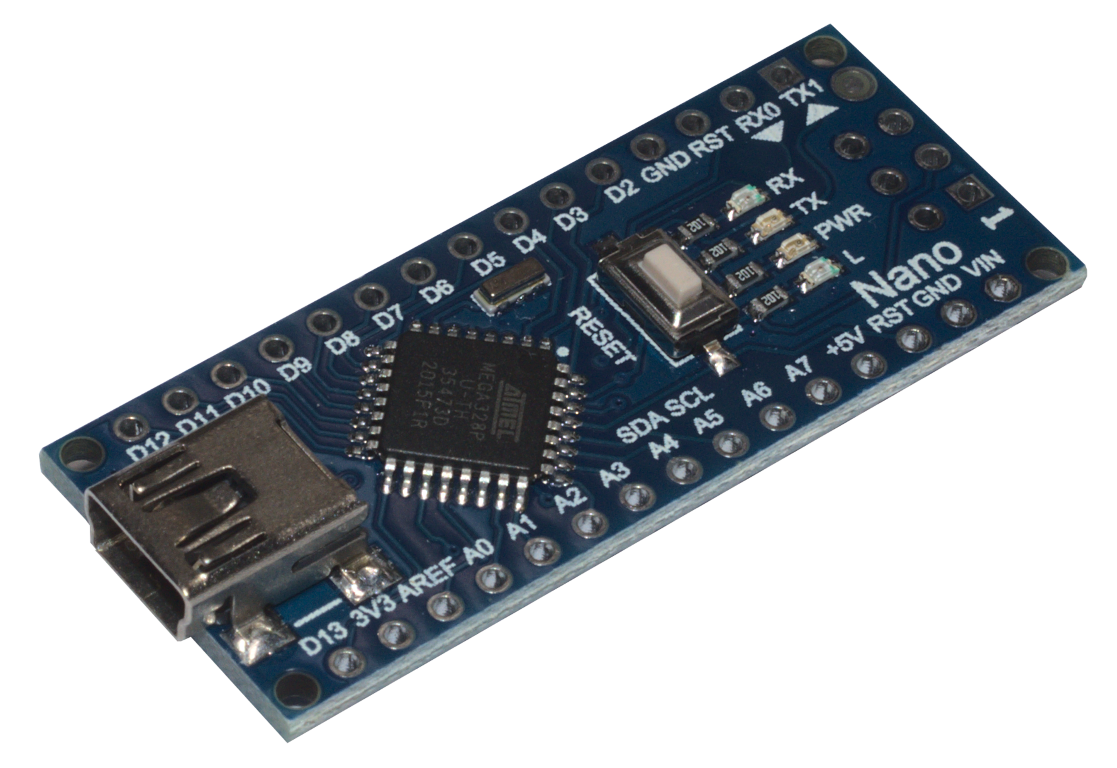
\includegraphics[width=\textwidth]{Fotos/Arduino_Nano.png}
\end{minipage}
\begin{minipage}{8cm}
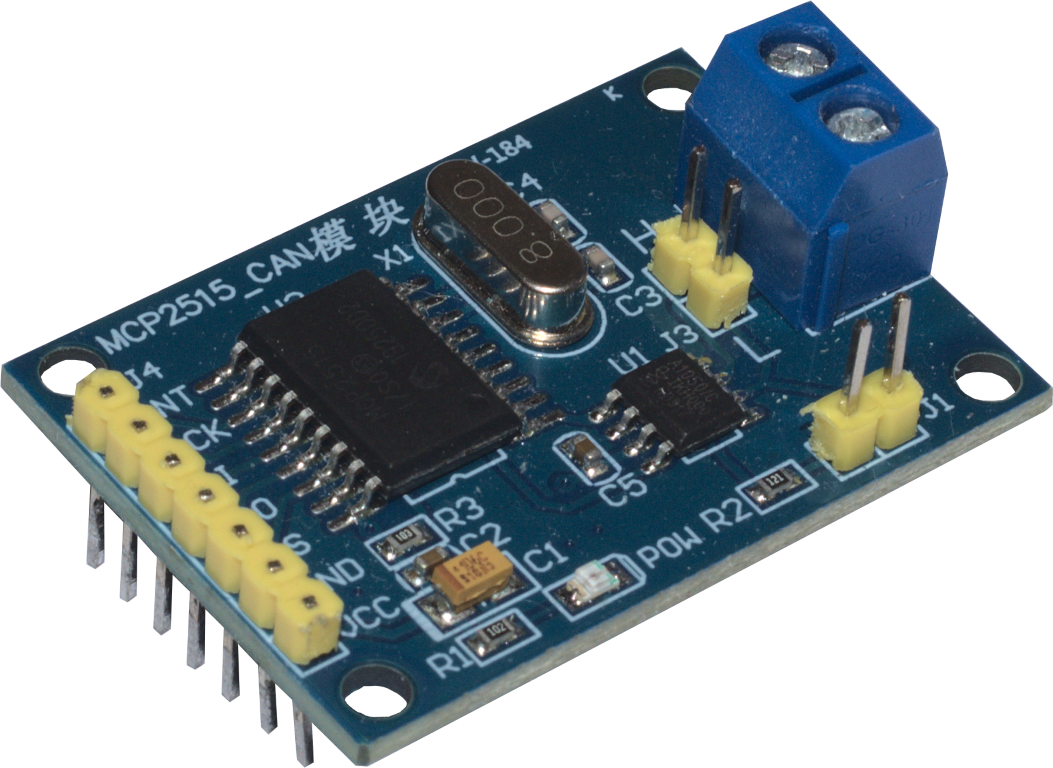
\includegraphics[width=\textwidth]{Fotos/CAN_BUS_Shield.png}
\end{minipage}
\section{Übertragungsmedium CAN-Bus}
Um eine zuverlässige Übertragung der Regelparameter für unsere Motoren sowie Servos garantieren zu können, wurde für deren Übertragung ein aus der Automobilbranche bekanntes Übertragungsmedium verwendet, der CAN-Bus. 
Neben seiner Robustheit trotz relativ hoher Übertragungsgeschwindigkeit, war es vorallem sein dezentraler Aufbau, der ihn für unseren Anwendungszweck optimal gemacht hat.
\todo[]{Verfeinerung des Textes, Bilder!}
\newpage
\section{Die zur Steuerung entworfenen Controller}
\subsection{Lenker}
Neben seiner Hauptaufgabe, nämlich dem Einlesen und der Übertragung der beiden Daumengas- sowie Lenkerstellungen ist dieser Mikrocontroller weiters für die Darstellung der von den verschiedenen Komponenten erhaltenen Telemetriedaten auf dem Bildschirm verantwortlich.
Dazu zählen neben den Informationen über die beiden Motoren vorallem auch die Temperaturen aller verbauten Akkus sowie die per GPS-Modul ermittelte derzeitige Geschwindigkeit.

\subsection{Motoren}
Diese wandeln die entsprechenden vom CAN-Bus übertragenen Daten mithilfe ihres 16-bit Timers (Timer1 des ATMEGA328p) in ein für unseren Motorregler verständliches PWM-Muster um.
Gleichzeitig übermitteln sie die von den Motorreglern übertragenen Telemetriedaten an den Controller des Lenkers.

\newpage
\subsection{Fahnen und Akkutemperaturen}
Auch die Ansteuerung der Servos erfolgte mit einem per CAN-Bus angeschlossenen Arduino. Um die für die Steuerung der drei Servos benötigten PWM-Signale unabhängig von den durch den Arduino bereitgestellten Timer und den damit verbunden GPIOs zu erzeugen 
(Anbindung des CAN-Bus Moduls über SPI benötigt beispielsweise diese Pins und Timer), wurde dafür auf ein externes Board zurückgegriffen.
Konkret handelt es sich um den \textbf{16-Channel 12-bit PWM/Servo Driver Driver} von Adafruit, welcher mittels I2C mit dem Mikrocontroller kommuniziert.\\

Die zweite Aufgabe dieses Controllers ist es, die Temperaturen aller acht im Boot verbauten Akkus zu überwachen, und diese zur Darstellung an den Controller des Lenkers zu übermitteln.
Dies geschieht mithilfe zweier (je einer pro Seite verbauten) ebenfalls über I2C verbundenen \textbf{ADS1115} Analog-Digital-Wandler, welche wiederum von Adafruit stammen.\\
Zur Temperaturmessung selbst kommt je ein \textbf{LM35} Temperatursensor pro Akku zum Einsatz.
\begin{figure}[h]
    \includegraphics[width=0.3\textwidth]{Fotos/ADS1115.png}
    \caption{ADS1115 Platinen}    
\end{figure}
\newpage
\section{Bildschirm}
Bei dem verwendeten Bildschirm handelt es sich um einen 5 Zoll großen Touchscreen aus dem Hause Nextion.
Diese bieten den großen Vorteil, die graphische Darstellung bequem über das verfügbare gratis Tool (\textbf{Nextion Editor}) designen zu können, während der Arduino den Bildschirm nur mit den nötigen Daten über eine Serielle Verbindung versorgen muss. 
